\documentclass[12pt]{article}

\usepackage[margin = .8in]{geometry}
\usepackage{amsmath}
\usepackage{graphicx}
\usepackage{multicol, enumerate, tabularx}

\usepackage{adjustbox, soul, setspace}

\usepackage[parfill]{parskip}

\usepackage{fancyhdr}
\pagestyle{fancy}

\lhead{Math F113X: Numbers and Society}
\rhead{Date: \hspace{1in}}

\usepackage{tikz}
\usetikzlibrary{calc,trees,positioning,arrows,fit,shapes,through, backgrounds}
\usetikzlibrary{patterns}

\usetikzlibrary{decorations.markings}
\usetikzlibrary{arrows}

\usepackage{pgfplots}

\usepackage{longtable}
\usepackage{tabularx}

\newcommand{\ds}{\displaystyle}
\newcommand{\ans}[1][1in]{\rule{#1}{.5pt}}

\newcommand{\points}[1]{(#1 points.)}		% Trying to be lazy.

\usepackage{array}
\newcolumntype{L}[1]{>{\raggedright\let\newline\\\arraybackslash\hspace{0pt}}m{#1}}
\newcolumntype{C}[1]{>{\centering\let\newline\\\arraybackslash\hspace{0pt}}m{#1}}
\newcolumntype{R}[1]{>{\raggedleft\let\newline\\\arraybackslash\hspace{0pt}}m{#1}}
\newcommand{\red}[1]{\textcolor{red}{#1}}

\newcommand{\be}{\begin{enumerate}}
\newcommand{\ee}{\end{enumerate}}

%\topmargin -1in
%\textheight 9.5in
%\oddsidemargin -0.3in
%\evensidemargin \oddsidemargin
%\pagestyle{empty}
%%\marginparwidth 0.5in
%\textwidth 7in
%\parindent 0in

%--------------------------------------------------------------------------------------------------------------------------------------------------------------------------
%						Document
%--------------------------------------------------------------------------------------------------------------------------------------------------------------------------


\begin{document}
%\pagestyle{fancy}
\begin{center}
{\Large  Worksheet 22 (Finance 2): Simple and Compound Interest}
\end{center}



\noindent \textbf{Group names:} \hrulefill \\
%-------------------------------------------------------------------------------------------------------------
%						Assignment
%-----------------------------------------------------------------------------------------------------
Recall:

\begin{tabular}{| l | l |}
\hline
$P$ = principal / starting amount & $r$ = annual interest rate (APR) \\ \hline
$I$ = interest & $n$ = number of compounding periods per year\\ \hline
$A$ = final amount & $t$ = number of years\\ \hline
\end{tabular}





\begin{tabular}{ c  c}
\fbox{Simple Interest} & \fbox{Compound Interest}\\
$A = P(1 + rt)$ & $A = P(1 + \frac{r}{n})^{nt}$
\end{tabular}

For the following problems, 

\be[(i)]

\item  Identify the value for each variable and which formula you should use

\item use a spreadsheet or a calculator to compute the quantities. 
\ee

For each quantity, carefully write \emph{what you need to compute} along with the answer.

To be efficient, you may want to write the following spreadsheet formula for compound interest (you would put in the correct numbers for each problem where it says [enter number]). You can fill down to compute $A$ for each problem.

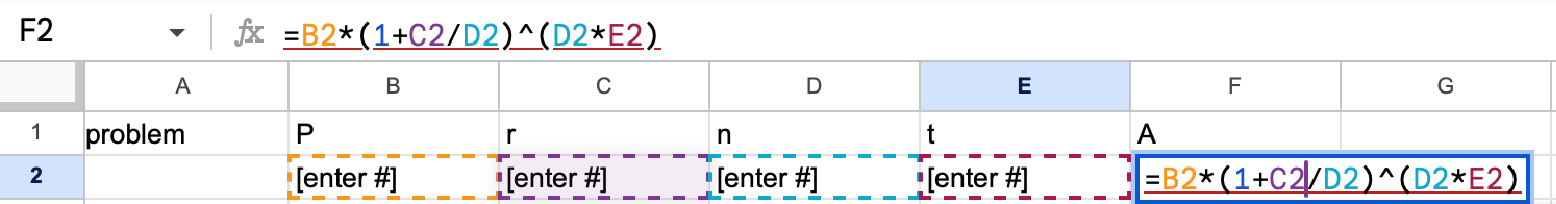
\includegraphics[width = \linewidth]{WS22-spreadsheetEx.pdf}

{\bf Example:} Your uncle gives you a simple interest loan of \$500 for one year, at 4\% annual interest. 

\be
\item How much interest do you owe?

\item What is the total amount you will owe him at the end of the year?
\ee

\fbox{
\parbox{\linewidth}{
Answer:

This is a simple interest problem. $P = 500$, $r = 0.04$, $t = 1$. 

(a) Total interest: $I = Prt = 500*0.04*1 = \$20$
 
(b) Final amount: $A = 500(1 + 0.04) = \$520$
}}

\begin{enumerate}

\item You borrowed \$1500 from a relative. 
\be
\item Suppose she charged you 5\% APR, compounded monthly. If you paid her back 5 years later, how much money did you give her?

\vfill

\item In the above situation, how much more interest did you pay than if she had charged you simple interest for 5 years?
\vfill
\ee

\newpage

\item You got a bonus of \$7,500 and you want to start a college fund for your child. You find an
account paying 9.75\% APR compounded quarterly. If your child just turned two years old,
how much will you have when they turn 18? How much of that account balance is interest?

\vfill

\item Calculate how much you would have in the previous problem if it was compounded
daily instead of quarterly. How much additional interest did you earn from the change in the number of compounding periods?

\vfill

\item If you are considering a credit card with an APR of 27.49\%, compounded daily, what
annual rate are you effectively paying? (To determine this, compute the total interest $I$ you paid for one year, and then compute $I/P$ and convert it into a percentage.)

\vfill

\item How much would you need to deposit today to have one million dollars if you can find an
account that pays 10\% interest, compounded daily, for 50 years?

Note that if $A = P(1 + \frac{r}{n})^{nt}$ then by algebra, $P = \frac{A}{(1 + \frac{r}{n})^{nt}}$.

\vfill


\newpage

\item For this problem, we want to compare simple interest to compound interest over time, in a graph.

Scenario: You put \$1000 on a credit card, which charges 20.4\% APR, compounded daily. Suppose this is an unrealistic credit card that does not have monthly minimum payments (we will talk about how to handle those later). 

\be
\item Make a new spreadsheet with spaces for $P$, $r$, $n$, and $t$ (which we will label ``years''). Make columns for compound interest and simple interest. I am showing you the formula for compound interest in the screenshot; you will need to modify it to enter simple interest.

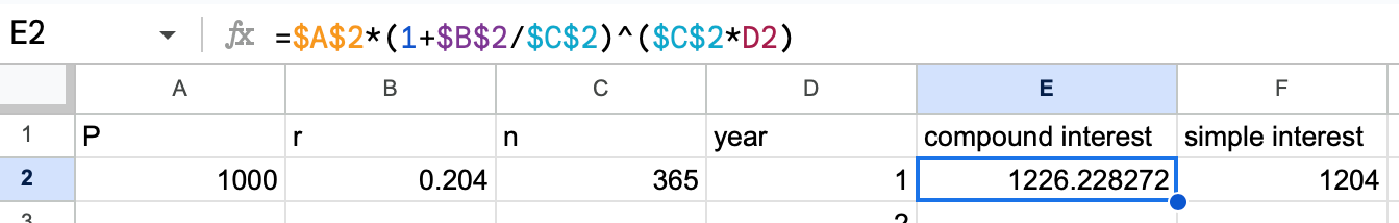
\includegraphics[width=\linewidth]{WS22-spreadsheetEx-2.pdf}



\item Fill down the ``year'' column by typing in 1 and 2, selecting both, and filling down until you reach 10 years. Then fill down the compound interest and simple interest columns.
\item Select the entries in the Compound Interest and Simple Interest columns, go to the {\tt Insert} column, select {\tt Chart}.
 
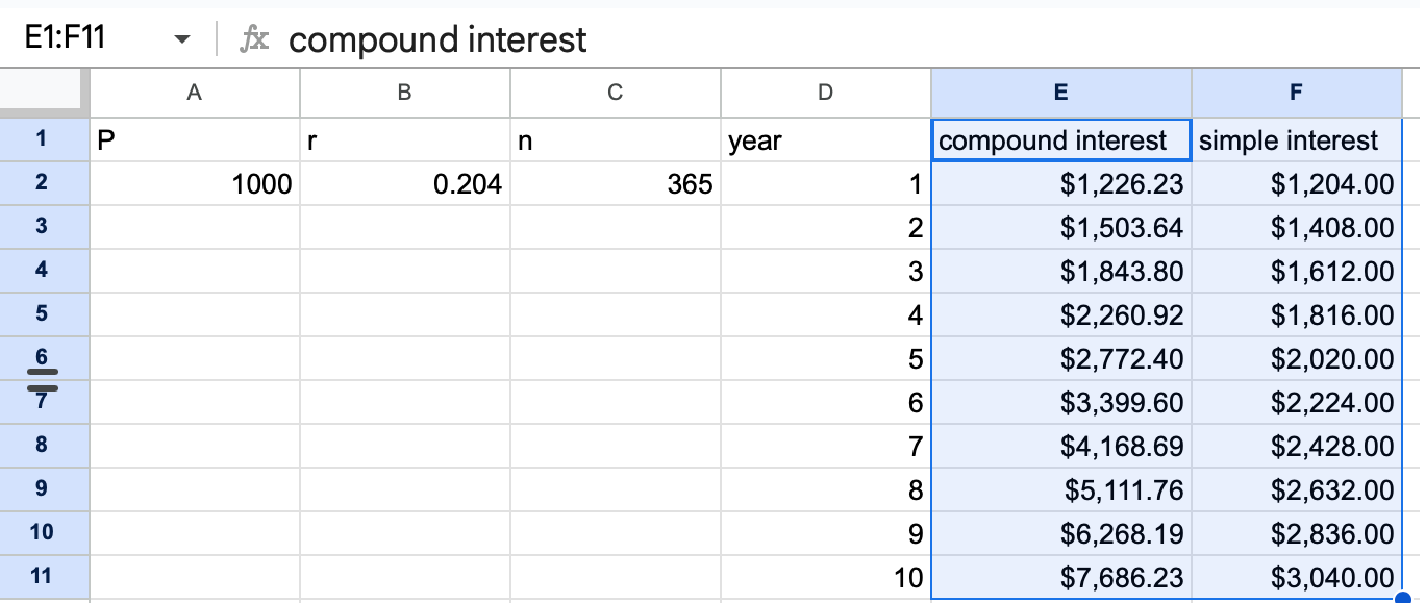
\includegraphics[width=.45\linewidth]{WS22-spreadsheetEx-3.pdf} \hfill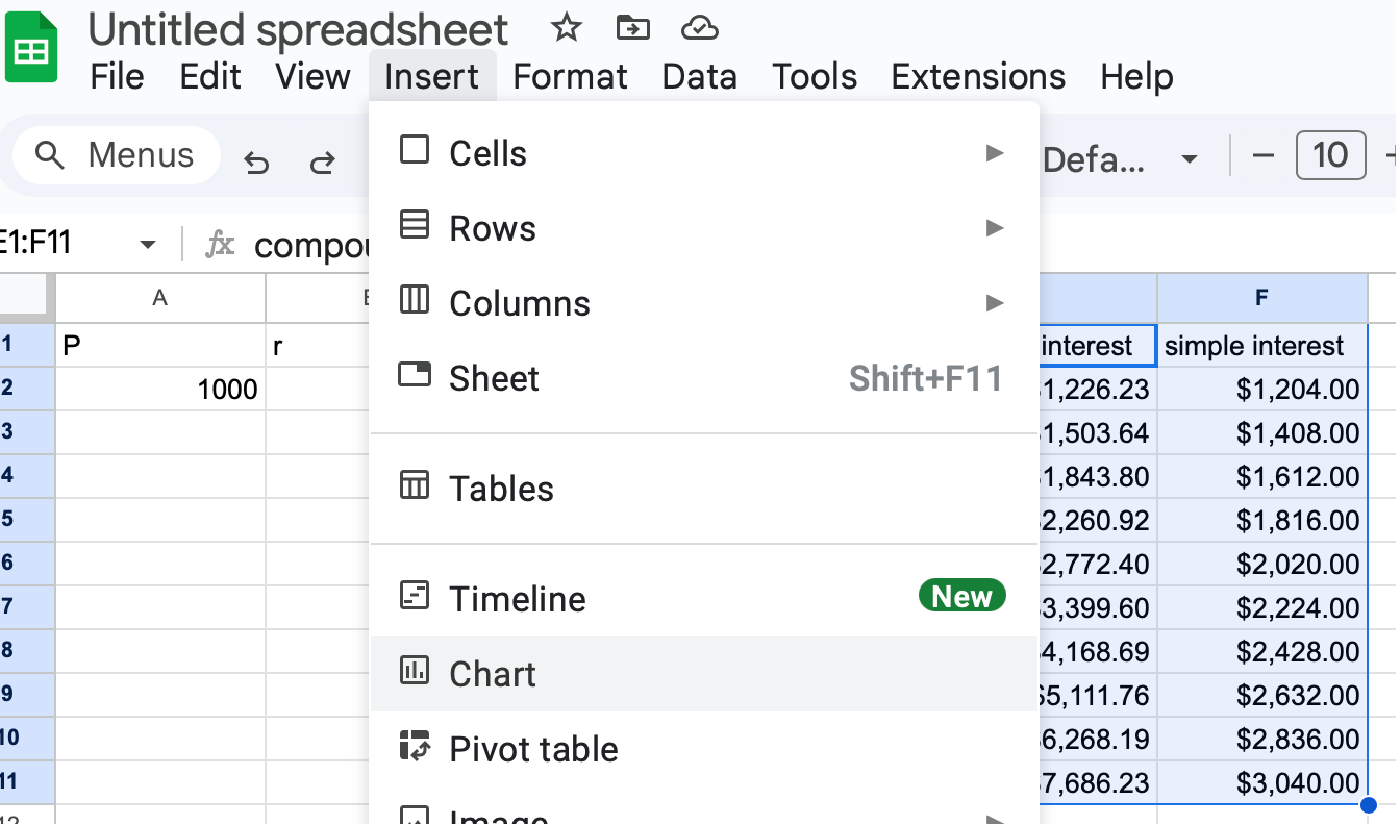
\includegraphics[width=.45\linewidth]{WS22-spreadsheetEx-4.pdf}


\item Move the chart so that you can see the chart and the data, and experiment with what happens to the chart if you change the number of compounding periods, or the interest rate. What do you notice?

\vfill

\item How much do you owe in interest at the end of 10 years? 

Simple interest: \ans 

 Compound interest: \ans
 \ee

\newpage

\item Modify the previous question to make a chart that shows the difference in interest if you compound \$1000 daily versus annually at 6\% annual interest rate for 100 years, looking at values every 10 years. You will need to have two different values for $n$ and two different compound interest columns.

What do you notice?
\vfill

\item Use a spreadsheet to answer the following question:

Alice deposited \$2498 into an account paying 7.05\% APR, compounded quarterly. Bob
deposited \$2994 into an account paying 5.19\% APR, compounded monthly. How many years
will it take for their balances to (nearly) match? 

\vfill

\item Which is better: an account that earns 7.25\% compounded quarterly, or an account that earns
7.15\% compounded daily? Give the effective rate (that is, the effective annual interest rate) for each account, and explain your answer
\vfill
\ee
\end{document}

%-------------------------------------------------------------------------------------------------------------------------------------------------------------------------------------------------------------------

%%% Local Variables:
%%% mode: latex
%%% TeX-master: t
%%% End:
